%*****************************************************************************%
% This LaTeX-Template is based on the beamer package:                         %
% http://latex-beamer.sourceforge.net                                         %
%                                                                             %
% For further details on how to create beamer slides you can check their      %
% documentation:                                                              %
% http://mirror.ctan.org/macros/latex/contrib/beamer/doc/beameruserguide.pdf  %
%                                                                             %
% The layout fits the current standard of the acg color scheme.               %
% Version: 1.0                                                                %
% Authors: Lars Krecklau <krecklau@informatik.rwth-aachen.de>                 %
%*****************************************************************************%
\documentclass{beamer}

\usepackage{graphicx}
\usepackage[german]{babel}

% Place in these lines your title and the author's names:
\newcommand{\myTitle}{Title}
\newcommand{\myAutors}{Authors}
\newcommand{\myAutorsFoot}{\myAutors}

% If you want to draw images by latex:
% http://www.texample.net/tikz/
\usepackage{tikz}
\usetikzlibrary{arrows,shapes}

% Apply the acg layout
\mode<presentation>
{
    \usetheme{Darmstadt}
    \useoutertheme{miniframes}
    \usecolortheme{acg}
    
    \setbeamercovered{transparent}
    \setbeamertemplate{navigation symbols}{}
    \setbeamertemplate{footline}
    {
        
\includegraphics[width=\paperwidth]{images/logo.png}
        \vspace*{-0.8cm}
        \begin{center}
            \color{ACGorange}\large{\insertpagenumber}
        \end{center}
        \vspace*{-0.8cm}
        \begin{flushright}
            \textcolor{ACGwhite}{\footnotesize{\myAutorsFoot}} \hspace*{0.95cm}
        \end{flushright}
        \vspace*{-0.3cm}
    }
    
    \setbeamertemplate{headline}
    {
        \vspace*{0.1cm}
        
\includegraphics[width=\paperwidth]{images/line.png}
        \vspace*{-0.1cm}
        \huge
        \begin{center}
            \invisible{Ag}
            \color{ACGorange}\insertsubsection
            \invisible{Ag}
        \end{center}
        \vspace*{-0.1cm}
        
\includegraphics[width=\paperwidth]{images/line.png}
        \vspace*{-0.3cm}
    }
}
 


% Setup the title page
\title{\myTitle}
\author{\myAutors}
\institute{RWTH Aachen University}
\date{\today}
\subject{\myTitle}

\begin{document}

\begin{frame}
    \titlepage
\end{frame}

\section{\myTitle}

\subsection{Layouts}

\begin{frame}[t]
    Start the content of the slide on top of the page...
\end{frame}

\begin{frame}
    ...or let it be centered automatically.
\end{frame}

\begin{frame}
    \begin{block}{Block 1}
        Use \textbf{blocks} to structure your slides.
    \end{block}
    \begin{block}{Block 2}
        Blocks will be aligned vertically.
    \end{block}
\end{frame}

\begin{frame}
    \begin{columns}[t]
    \column[T]{0.7\linewidth}
        \begin{block}{Block 1}
            Use \textbf{columns} for horizontal slide layouts
        \end{block}
        \begin{block}{Block 2}
            Blocks will be vertically aligned in each column
        \end{block}
    \column[T]{0.3\linewidth}
        \begin{block}{Block 3}
            \begin{figure} 
                \centering 
                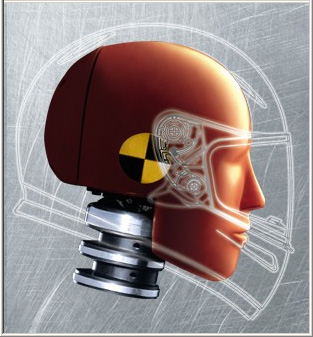
\includegraphics[width=\linewidth]{images/dummy}
            \end{figure}
        \end{block}
    \end{columns}
\end{frame}

\subsection{Beamer Techniques}

\begin{frame}
    \begin{block}{Uncover}
        \begin{itemize}
            \item Use \textbf{uncovering} for making only parts of the slide fully visible
            \uncover<2->{\item This helps to concentrate on the current points}
        \end{itemize}
    \end{block}
\end{frame}

\begin{frame}
    \begin{block}{Alert}
        \begin{itemize}
            \item Use \textbf{alert} as another technique for emphasizing
            \uncover<2->{\item Focus on \alert<2>{important} details}
            \uncover<3->{\item This helps to guide the viewer through your presentation}
        \end{itemize}
    \end{block}
\end{frame}

\begin{frame}
    \begin{block}{Visible}
        \begin{itemize}
            \item You may also want to place something in between points
            \visible<2>{\item So this is our additional information}
            \item But already reserve the space
        \end{itemize}
    \end{block}
\end{frame}

\begin{frame}[t]
    \begin{columns}[t]
    \column[T]{0.7\linewidth}
        \begin{block}{Only}
            \begin{itemize}
                \item Use \textbf{only} to display something on one specific slide
                \item For example: Images to certain keypoints:
                \begin{itemize}
                    \uncover<2->{\item Image on \alert<2->{\only<-2>{100}\only<3>{50}\only<4>{25}\%} line width}
                \end{itemize}
            \end{itemize}
        \end{block}
    \column[T]{0.3\linewidth}
        \only<2->{
            \begin{block}{Image}
                \only<2>{
                    \begin{figure} 
                        \centering 
                        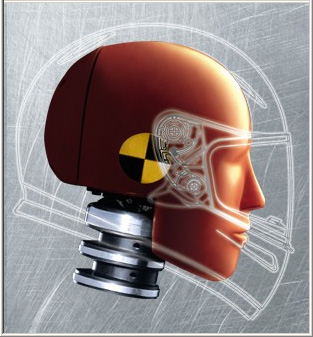
\includegraphics[width=\linewidth]{images/dummy}
                    \end{figure}
                }
                \only<3>{
                    \begin{figure} 
                        \centering 
                        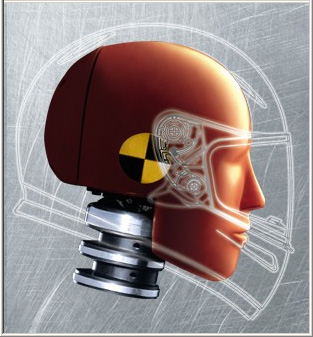
\includegraphics[width=0.5\linewidth]{images/dummy}
                    \end{figure}
                }
                \only<4>{
                    \begin{figure} 
                        \centering 
                        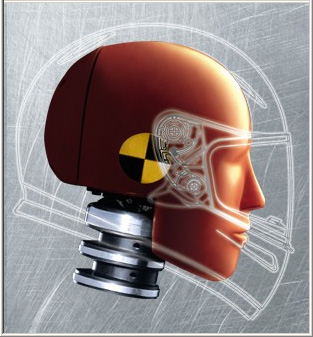
\includegraphics[width=0.25\linewidth]{images/dummy}
                    \end{figure}
                }
            \end{block}
        }
    \end{columns}
\end{frame}

\subsection{TikZ + Beamer}

\begin{frame}
    % Example taken from: http://www.texample.net/tikz/examples/beamer-arrows/
    % The example was slightly modified
    \begin{block}{Use TikZ in LaTeX}
        % For every picture that defines or uses external nodes, you'll have to
        % apply the 'remember picture' style. To avoid some typing, we'll apply
        % the style to all pictures.
        \tikzstyle{every picture}+=[remember picture]

        % Below we mix an ordinary equation with TikZ nodes. Note that we have to
        % adjust the baseline of the nodes to get proper alignment with the rest of
        % the equation.        
        \begin{equation*}
        \vec{a}_p = \vec{a}_o+\frac{{}^bd^2}{dt^2}\vec{r} +
            \tikz[baseline]{
                \node[draw, anchor=base] (t1)
                {$ 2\vec{\omega}_{ib}\times\frac{{}^bd}{dt}\vec{r}$};
            } +
            \tikz[baseline]{
                \node[draw, anchor=base] (t2)
                {$\vec{\alpha}_{ib}\times\vec{r}$};
            } +
            \tikz[baseline]{
                \node[draw,anchor=base] (t3)
                {$\vec{\omega}_{ib}\times(\vec{\omega}_{ib}\times\vec{r})$};
            }
        \end{equation*}

        \begin{itemize}
            \alert<1>{\item Coriolis acceleration}    \tikz[baseline=-.5ex] \node [coordinate] (n1) {};
            \alert<2>{\item Transversal acceleration} \tikz[baseline=-.5ex] \node [coordinate] (n2) {};
            \alert<3>{\item Centripetal acceleration} \tikz[baseline=-.5ex] \node [coordinate] (n3) {};
        \end{itemize}

        % Now it's time to draw some edges between the global nodes. Note that we
        % have to apply the 'overlay' style.
        \begin{tikzpicture}[overlay]
            \path[->]<1-> (n1) edge [bend right]    (t1);
            \path[->]<2-> (n2) edge [bend right]    (t2);
            \path[->]<3-> (n3) edge [out=0, in=-90] (t3);
        \end{tikzpicture}
    \end{block}
\end{frame}

\end{document}